\chapter{Programmazione Dinamica - DP}
La programmazione dinamica (DP - Dynamic Programming) è una tecnica che (come il Divide et Impera),
risolve i problemi combinando le soluzioni dei sottoproblemi.\\
Divide et Impera è ottimo quando i sottoproblemi da risolvere sono indipendenti,
mentre DP è efficace quando i sottoproblemi non sono indipendenti e quindi hanno in comune
dei sottosottoproblemi e le tecniche di risoluzione top-down risultano quindi inefficienti (chiamate ripetute).
La programmazione dinamica si applica tipicamente ai \textbf{problemi di ottimizzazione}.
\section{Problemi di ottimizzazione}
Sono problemi dove ci sono molte soluzioni possibile. Ogni soluzione ha un valore e e si vuole trovare una solzuione
con il valore  ottimo. Ci possono essere più soluzioni che raggiungono il valore ottimo.
\section{Il processo di sviluppo}
Il processo di sviluppo è diviso in 4 fasi:
\begin{itemize}
    \item Caratterizzare la struttura di una soluzione ottima
    \item Definire in modo ricorsivo il valore di una soluzione ottima
    \item Calcolare il valore di una soluzione ottima, di solito con uno schema bottom-up (dal basso verso
    l'alto, risulta spesso più efficiente rispetto a top-down)
    \item Costruire una soluzione ottima dalle informazioni calcolate
\end{itemize}
\section{Esempio - Fibonacci}
Classico esempio è l'esecuzione di Fibonacci. Utilizzando la ricorsione pura
si effettuano più volte le stesse chiamate (perchè i sotto-numeri sono gli stessi). Se invece
utilizziamo la DP, con un approccio Bottom-Up ci dobbiamo chiedere,
ma chi è Fibonacci di n? è Fibonacci di (1)+Fibonacci(2)+ ... + Fibonacci(n). In pratica
inizio a calcolare le soluzioni dal sottoproblema più piccolo a salire, così facendo possiamo risparmiare molto tempo,
al costo però di un maggiore utilizzo di spazio, dato che ho un Array che deve memorizzare i valori. Si tratta 
di un compromesso accettabile dato che senza usare Array il tempo di esecuzione sarebbe esponenziale.
\subsection{Passaggi}
A livello pratico dobbiamo:
\begin{enumerate}
    \item Scomporre il problem in sottoproblemi di dimensione inferiore
    \item Formulare la soluzione in maniera ricorsiva - Equazioni di Ricorrenza
    \item Usare una strategia bottom-up (non top-down)
    \item Memorizzare i risultati in una opportuna struttura dati
    \item Individuare il "luogo" che contiene la soluzione del problema (nel caso di Fibonacci l'ultima cella a destra)
\end{enumerate}
DP risulta vantaggiosa quando il numero di chiamate distine è polinomiale (il numero
totale di chiamate è esponenziale).
\section{Osservazioni sui problemi di ottimizzazione}
Per ogni istanza del problema esiste un insieme di soluzioni posibili (feasible solutions),
più soluzioni perchè le soluzioni ottime possono essere diverse.\\
Esiste una funzione obiettivo che associa un valore ad ogni soluzione possibile e
restituisce come OUTPUT una soluzione possibile (soluzione ottimale) per cui il valore restituito dalla funzione
obiettivo è massimo/minimo (valore ottimo).

\section{LCS - Longest Common Subsequence}
Si tratta di un problema che ha come istanza due sequenze di valori e richiede di trovare la 
più grande sottosequenza comune fra di esse. Si tratta di un problema di ottimizzazione, per questo
usare DP è un'ottima idea.
\subsection{Definizioni di base}
\paragraph*{Sequenza} Successione di elementi topologicamente ordinati, presi da un insieme
$\sum$.\\
Per esempio $X=<2,4,10,5,9,11>$, più in generale:
\begin{itemize}
    \item $X=<x_1, x_2, ..., x_m> \rightarrow$ sequenza di $m=|X|$ elementi
\end{itemize}
\paragraph*{Prefisso di lunghezza i} Primi i elementi della sequenza:
\begin{itemize}
    \item $X=<x_1, x_2, ..., x_i> \rightarrow$ prefisso di lunghezza i di X
\end{itemize}
Dato $X=<2,4,10,5,9,11>$ per esempio $X_3=<2,4,10>$.
\paragraph*{i-esimo elemento} Indichiamo con $X[i]$ l'i-esimo elemento $x_i$ della sequenza X.
\paragraph*{Sottosequenza} Una qualsiasi successione di elementi (anche non consecutivi)
di una sequenza che però rispettino l'ordine sulla sequenza.\\
Per esempio data una sequenza $X=<2,4,10,5,9,11>$ 
\begin{itemize}
    \item $Z=<4,5,9>$ è una sottosequenza di X
    \item $Z=<>=\epsilon$ è una sottosequenza di X
    \item $<9, 5, 4>$ NON è una sottosequenza di X
\end{itemize}
\paragraph*{Definizione formale di sottosequenza}
Data $X = <x_1, x_2, ..., x_m>$, una sequenza $Z=<z_1, z_2, ..., z_k>\, (k \leq m)$ è
sottosequenza di X se esiste una successione di k indici interi $i_1 < i_2 < .. < i_k$ tali che
$X[i_j] = z_j$ per j compreso tra 1 e k.
\paragraph*{Esempio sottosequenza} Dato $X=<2,4,10,5,9,11>$, $Z=<4,5,9>$ è una sottosequenza di X.
\paragraph*{Sottosequenza comune di X e Y} è una sottosequenza si di X che di Y.
\[X = <1, 13, 5, 3, 1, 12, 8, 11, 6, 10, 10>\]
\[Y = <1, 5, 5, 2, 3, 1, 12, 8, 8, 10>\]
\[S = <5, 3, 1, 8, 10>\]\\
S è sottosequenza comune di X e Y.
\paragraph*{LCS} è la più lunga sottosequenza comune Z di X e Y.
\paragraph*{Esempio di LCS}
\[X = <2, 10, 5, 3, 1, 12, 8, 30, 11, 6, 10, 13>\]
\[Y = <2, 5, 10, 2, 3, 1, 30, 12, 6, 8, 10>\]
\[<2, 10, 3, 1, 12, 8, 10> \text{è LCS di X e Y}\]
La LCS è una soluzione ottimale, mentre la sua lunghezza (7) è il valore ottimo.\\
\subsection{Istanza del problema}
P: date due sequenze $X = <x_1, x_2, ..., x_n> e Y = <y_1, y_2, ... , y_n>$, trovare la più lunga
sottosequenza comune Z di X e Y.\\
Abbiamo capito che P è un problema di ottimizzazione di massimo, dove:
\begin{itemize}
    \item (m,n) $\rightarrow$ è la dimensione del problema (lunghezza stringhe)
    \item Soluzioni possibili $\rightarrow$ tutte le sottosequenze comuni di X e Y
    \item Funzione obiettivo $\rightarrow$ lunghezza
    \item $|Z|$ è il valore ottimo del problema
    \item Z è una soluzione ottimale
\end{itemize}
\section{Procedura LCS}
Indichiamo con LCS(A,B) la LCS delle sequenze A e B e di conseguenza $|LCS(A,B)|$
 la lunghezza della LCS di A e B.\\
 Procediamo con le seguenti fasi:
 \begin{enumerate}
    \item Individuiamo i sottoproblemi
    \item Troviamo le equazioni di ricorrenza
    \item Applichiamo una strategia bottom-up con memorizzazione dei risultati
 \end{enumerate}
 \paragraph*{Nota Bene} Si deve individuare la sottostruttura ottima del problema. La strategia bottom-up trova
 l'ottimo (lunghezza di LCS) e in seguito si deve ricostruire una soluzione ottimale (una delle LCS).
 \subsection{Definizione dei sottoproblemi}
 Sottoproblema di dimensione (i,j).
 Trovare la LCS dei prefissi $X_i$ e $Y_j \rightarrow LCS(X_i, Y_j)$.
 \[i \in \{0,1, ..., m\}\]
 \[j \in \{0,1,...,n\}\]
 Numero totale sottoproblemi: $(m+1)\times(n+1)$\\
 Ricordiamo che $LCS(X_m,Y_n)$ è la soluzione del problema principale.
 \subsection{Equazioni di ricorrenza}
 \subsection*{Casi base}
 Tutti i sottoproblemi di dimensione (i,j) tale per cui $i=0$ oppure $j=0$.
\begin{align*}
    i= 0 \implies LCS(X_0, Y_j) = LCS(\epsilon, Y_j) = \epsilon \\
    j = 0 \implies LCS(X_i, Y_0) = LCS(X_i, \epsilon) = \epsilon \\
    i = 0,\, j=0 \implies LCS(X_0, Y_0) = LCS(\epsilon, \epsilon) = \epsilon
\end{align*}
\subsection*{Passo ricorsivo}
Tutti i sottoproblemi di dimensione (i, j) tale per cui $i>0$ e $j>0$.\\
Introduciamo la sottostruttura ottima del problema:
\paragraph*{Esempio di sottostruttura ottima}
\begin{align*}
    &X= <(3, 5, 4, 3, 10, 12, 8, 30)> \quad m=8\\
    &Y = <(3, 2, 4, 10, 2, 8, 30, 13, 30)> \quad n=9
\end{align*}
LCS(X,Y) $\rightarrow Z = <z_1, z_2, \dots, z_{k-1}, z_k> = <3,4,10,8,30>$.\\
Sicuramente $z_k=30$. Come mi comporto per $k-1$? $z_1, z_2, ..., z_{k-1}> \rightarrow LCS(?,?)?$.\\
Avrò sicuramente che sarà la LCS di $(k-1)+30$, quindi:
\[LCS(X,Y)=LCS(X_7, Y_8) + <30>\]
\subsection{Sottostruttura ottima}
Date:
\begin{itemize}
    \item $X=<x_1, x_2, \dots, x_{m-1}, x_m>$
    \item $Y=<y_1, y2_, \dots, y_{n-1}, y_n>$ 
    \item $LCS(X, Y) = <z_1, z_2, \dots, z_{k-1}, z_k>$
\end{itemize}
La sottostruttura ottima sarà data da:\\
$x_m = y_n \implies \, LCS(X,Y) = LCS(X_{m-1},Y_{n-1})+<x_m>$
\begin{enumerate}
    \item $z_k = x_m = y_n$
    \item $<z_1, z_2, \dots, z_{k-1}> = LCS(X_{m-1}, Y_{n-1})$
\end{enumerate}
$x_m \neq y_n \implies = max\{LCS(X_{m-1}, Y_n), LCS(X_m, Y_{n-1})\}$
\begin{enumerate}
    \item $z_k \neq x_m \implies LCS(X,Y)=LCS(X_{m-1},Y_n)$
    \item $z_k \neq y_n \implies LCS(X,Y)=LCS(X_m, Y_{n-1})$
\end{enumerate}
\subsection{Equazioni di ricorrenza}
\paragraph*{i=0 $\vee$ j = 0 (CASI BASE)}
\begin{align*}
    LCS(X_i, Y_j) = \epsilon
\end{align*}
\paragraph*{$i > 0 \wedge j>0$ (PASSO RICORSIVO)}
\begin{align*}
    &x_i = y_j \implies LCS(X_i, Y_j) = LCS(X_{i-1}, Y_{j-1}) + <x_i>\\
    &x_i \neq y_j \implies LCS(X_i, Y_j) = max\{LCS(X_{i-1}, Y_j), LCS(X_i, Y_{j-1})\}
\end{align*}
\subsection*{Applichiamo la funzione "lunghezza" alle equazioni}
La funzione lunghezza è definita come segue:
\[c_{i,j} = |LCS(X_i, Y_j)|\]
\paragraph*{i=0 $\vee$ j = 0 (CASI BASE)}
\begin{align*}
    |CS(X_i, Y_j)| = |\epsilon| = 0
\end{align*}
\paragraph*{$i > 0 \wedge j>0$ (PASSO RICORSIVO)}
\begin{align*}
    &x_i = y_j \implies |LCS(X_i, Y_j)| = |LCS(X_{i-1}, Y_{j-1})| + |<x_i>|\\
    &x_i \neq y_j \implies |LCS(X_i, Y_j)| = max\{|LCS(X_{i-1}, Y_j)|, |LCS(X_i, Y_{j-1})|\}
\end{align*}
\subsection*{Calcoliamo la lunghezza di ciò che è noto}
\paragraph*{i=0 $\vee$ j = 0 (CASI BASE)}
\begin{align*}
    c_{i,j} = 0
\end{align*}
Dato che ho i=0 e j=0.
\paragraph*{$i > 0 \wedge j>0$ (PASSO RICORSIVO)}
\begin{align*}
    &x_i = y_j \implies c_{i,j} = c_{i-1,j-1} + 1
    &x_i \neq y_j \implies c_{i,j} = max\{c_{i-1,j}, c_{i,j-1}\}
\end{align*}
Dato che $<x_i>$ è un singolo carattere, quindi ha lunghezza 1. Le sostituzioni
delle funzioni LCS sono la semplice sostituzione della definizione di funzione lunghezza
sopra riportata.
\paragraph*{Quanti coefficienti/variabili $c_{i,j}$?} (m+1)(n+1) coefficienti/variabili.
\paragraph*{$c_{m,n}$} $=|LCS(X_m, Y_n)| = |LCS(X,Y)|$, 
\textbf{è il valore ottimo del problema principale}.
\subsection*{Soluzione del problema}
\begin{itemize}
    \item Calcolo del valore ottimo (top-down oppure bottom-up?)
    \item Ricostruzione di una soluzione ottimale
\end{itemize}
Perchè io tramite la procedura effettuo il riempimento della matrice, devo capire quindi dove
si trova il valore (in questo caso abbiamo visto in $c_{m,n}$) e devo ricostruire la
sottosequenza dato che la matrice contiene lunghezze, non stringhe.
\paragraph*{Proviamo con una strategia top-down}
\begin{lstlisting}[language=Java, escapeinside={*@}{@*}]
    int ottimo-ricorsivo(i,j)
        if i = 0 || j = 0 then
            return 0
        else
            if *@$x_i = y_j$@* then
                *@$c_{i,j}$@* = ottimo-ricorsivo(i-1,j-1)+1
                return *@$c_{i,j}$@*
            else
                *@$c_{i-1,j}$@* = ottimo-ricorsivo(i-1,j)
                *@$c_{i,j-1}$@* = ottimo-ricorsivo(i,j-1)
                return max{*@$c_{i-1,j},c_{i,j-1}$@*}
\end{lstlisting}
Valore ottimo $\rightarrow$ ottimo-ricorsivo(m,n).
\paragraph*{Complessità in tempo nel caso migliore?} $\Omega(n)$ nel caso migliore in cui $X=Y$ e
$|X|=n$.\\
\paragraph*{Complessità in tempo nel caso peggiore?} Esponenziale, perchè continua a creare dei
rami per testare la stringa diminunedo di 1 prima a sinistra e poi a destra. Quindi non è una
buona idea in questo caso applicare questa strategia.

\subsection{Riassumendo - Per calcolare l'ottimo}
\begin{enumerate}
    \item Definizione dei sottoproblemi
    \item Equazioni di ricorrenza
    \begin{itemize}
        \item Casi base
        \item Passo ricorsivo (sottostruttura ottima)
    \end{itemize}
    \item Definizione dei coefficienti/variabili (valori ottimi dei sottoproblemi)
    \item Individuazione del coefficiente ottimo (valore ottimo dle problema principale)
    \item Equazioni di ricorrenza in termini dei coefficienti
    \item Calcolo dei coefficienti seguendo una strategia bottom-up
    \item Determinazione del valore ottimo
\end{enumerate}
\subsection{Dimostrazione matematica per assurdo della sottostruttura ottima}
Attualmente non ho molta sbatti di trascriverla, quindi rimanderò a domani o dopo questa
infausta operazione.
%AGGIUNGERE DIMOSTRAZIONI SLIDE 15-41 (LCS - Equazioni di Ricorrenza)
\subsection{Risoluzione Bottom-Up}
\begin{itemize}
    \item Si calcolano i coefficienti $c_{i,j}$ per dimensione $(i,j)$ crescente
    a partire dai casi base $(0,j)$ e $(i,0)$
    \item Si memorizza $c_{i,j}$ ogni volta che si risolve il sottoproblema $(i,j)$
    \item Quando si arriva a calcolare $c_{m,n}$ si ha il valore ottimo
\end{itemize}
\paragraph*{Algoritmo DP (bottom-up)}
\begin{enumerate}
    \item Si costruisce una matrice C di m+1 righe e n+1 colonne
    \item Si indicizzano le righe e le colonne a partire da 0
    \item Si riempie C in modo tale che $C[i,j] = c_{i,j}$
    \item Valore ottimo si trova in $C[m,n] = c_{m,n}$
\end{enumerate}
\subsubsection*{Matrice}
\begin{center}
    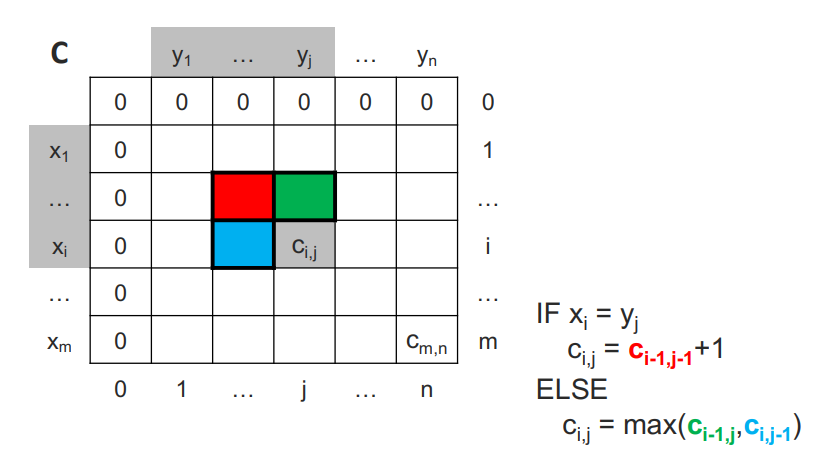
\includegraphics[width=70mm,scale=0.5]{chapters_ulerich/img/LCS_matrix.png}
\end{center}
Notiamo subito che la prima riga e prima colonna vengono inizializzate a 0, dato che
la LCS tra una qualsiasi sequenza e una nulla è 0.
\subsection*{Codice riempimento matrice}
\begin{lstlisting}[language=Java, escapeinside={*@}{@*}]
int ottimo_DP(X,Y)
    for i from 0 to m do
        C[i,0] = 0
    for j from 0 to n do
        C[0,j] = 0
    for i from 1 to m do
        for j from 1 to n do
            if *@$x_i = y_j$@* then
            C[i,j] = C[i-1,j-1] + 1
        else
            C[i,j] = max(C[i-1,j],C[i,j-1])
    return C[m,n]
\end{lstlisting}
\paragraph*{Complessità in tempo} $\Theta (mn)$
\paragraph*{Esempio di matrice riempita}
\begin{center}
    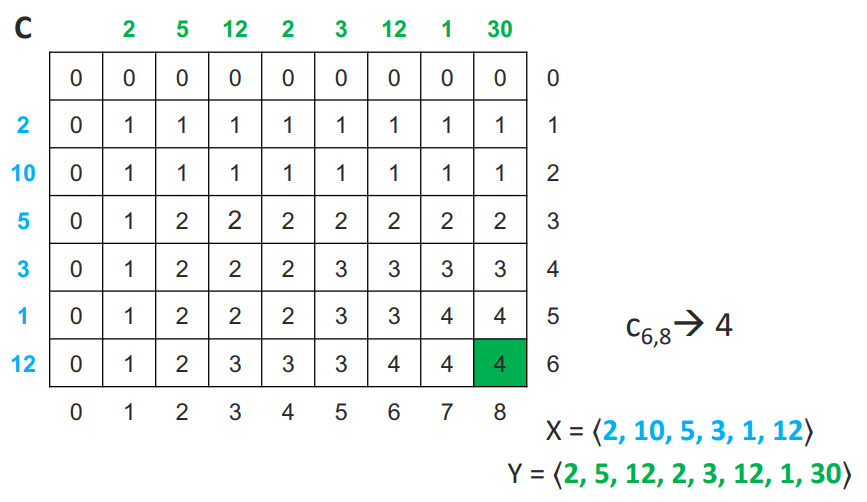
\includegraphics[width=90mm, scale=0.5]{chapters_ulerich/img/LCS_matrix_riempita.png}
\end{center}
\subsection{Ricostruzione della soluzione ottimale}
Ora che abbiamo la matrice dei coefficienti abbiamo la LCS, o meglio il valore della
LCS (quanto è lunga la più lunga sottosequenza di caratteri in comune fra le 2 sequenze), ma
non abbiamo la stringa! \'E necessario ricostruire tramite la matrice la mia soluzione ottimale.
\paragraph*{La procedura} Partiamo dall'ultima cella in basso a destra (cella del valore ottimo),
che nell'esempio riporta il valore di 4:\\
Dobbiamo scegliere fra 3 possibili celle dove spostarci:
\begin{itemize}
    \item La cella sinistra - Se contiene il valore maggiore fra i 3
    \item La cella in alto - Se contiene il valore maggiore fra i 3
    \item La cella diagonale - Se le celle hanno lo stesso valore decrementato di 1 rispetto a
    quello della cella di partenza
\end{itemize}
Quando mi muovo in diagonale salvo il carattere di riferimento della colonna (o riga, tanto saranno uguali) e proseguo
con la procedura.\\
La procedura consiste nel calcolare la LCS guardando i coefficienti della matrice.\\
\paragraph*{Inizio ricostruzione} Partendo da 4 mi chiedo: Quale è la $LCS(X_6, Y_8)$? Guardo i coefficienti della matrice, quale valore fra 4, 4 scelgo? Qua non posso andare in diagonale perchè 
non ho un decremento del coefficiente di 1, posso andare solo a sinistra o in alto. Scelgo per esempio
di andare a sinistra. Non essendoci stato un decremento del coefficiente (infatti non ho valori uguali sugli indici della
matrice), non ho un carattere appartenente alla soluzione ottima, quindi avrò $LCS(X_6, Y_8) = LCS(X_6, Y_7)$,
quindi mi sposto e cerco la $LCS(X_6, X_7)$.
\begin{center}
    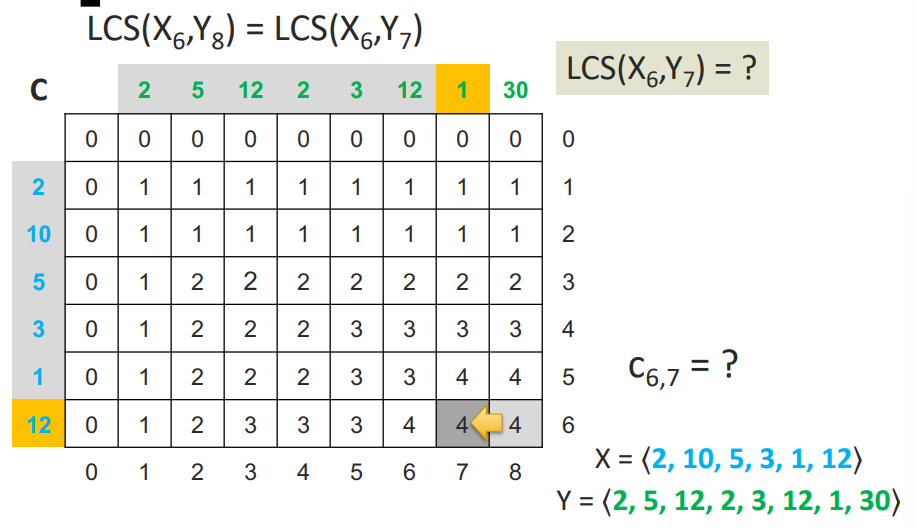
\includegraphics[width=90mm,scale=0.5]{chapters_ulerich/img/LCS_matrix_ricostruzione_sol_ottima.png}
\end{center}
Nel caso in cui la cella di partenza e le altre 3 fossero uguali si può scegliere di andare
o in alto o a sinistra, si ottiene comunque la stessa soluzione, nel caso in cui si ottengono spostamenti
diagonali differenti significa che si avrà un'altra soluzione ottima.\\
Proseguo e noto che anche qua ho due coefficienti uguali, scelgo di andare in alto, 
$LCS(X_6, X_7) = LCS(X_5, Y_7)$.
\paragraph*{Osservazione} Se fossi andato a sinistra al passaggio successivo avrei avuto un passaggio a una 
diagonale che non percorrerò andando in alto, questa è un'altra soluzione ottima.\\
Ora mi trovo a calcolare $LCS(X_5, X_7)$. Qua ho tutti e 3 i valori uguali decrementati di 1, 
posso effettuare uno spostamento diagonale! Si tratta di un carattere della soluzione ottima quindi avrò che:
\begin{align*}
    &c_{5,7} = c_{4,6} + 1\\
    &LCS(X_5,Y_7) = LCS(X_4, Y_6) + <x_5>\\
    &LCS(X_6,Y_8) = LCS(X_5,Y_7)\\
    &LCS(X_6,Y_8) = LCS(X_4,Y_6) + <x_5>\\
    &LCS(X_6,Y_8) = LCS(X_4,Y_6) + <1>
\end{align*}
Dove 1 è l'ultimo carattere della LCS.\\
Proseguo a ritrovo fino a quando arriverò in cima alla matrice e avrò il caso base $LCS(X_0, Y_0) = \epsilon$.\\
Ora ho la sottosequenza ottima!\\
\subsection{Algoritmo ricorsivo ricostruzione soluzione ottima}
\paragraph*{Input} Matrice C e indici i e j di una cella di C.
\paragraph*{Output} Una soluzione ottimale per i prefissi $X_i$ e $Y_j$.

